% Main-manuscript figures, in their numerical order. Algorithms remain in the Methods section.
% Every figure is drawn by the talk's figure code from the talk's data files (figs/src/build_figs.sh); the data
% files are written by scripts/30_talk_data.jl from the committed results.

% talk/data/market_state.csv, talk/data/market_state_crossings.csv
\begin{figure}[H]
    \centering
    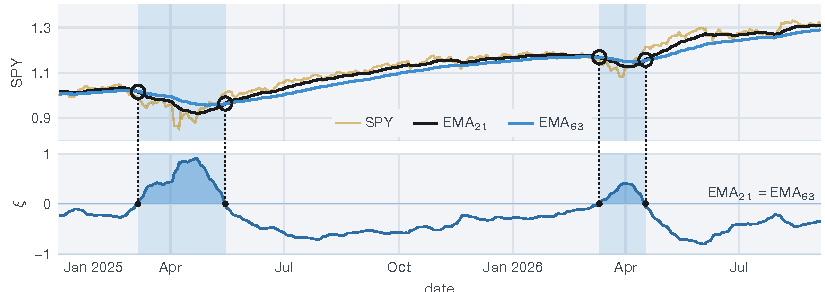
\includegraphics[width=\textwidth]{figs/main/fig_market_state.pdf}
    \caption{\textbf{SPY and the market state over the trading window, 2 January 2025 to 4 September 2026.}
    Top: SPY's daily close (light gold) with its $21$-day (black) and $63$-day (blue) exponential moving averages
    (EMAs), each divided by SPY's first close in the window. Bottom: the market state
    $\xi = -G(\mathrm{EMA}_{21}/\mathrm{EMA}_{63} - 1)$, where the gain $G = 21.23$ is the reciprocal of the $99$th
    percentile of $\lvert \mathrm{EMA}_{21}/\mathrm{EMA}_{63} - 1 \rvert$ over 2014--2024. Its positive part is filled. Shaded days have $\xi > 0$,
    when the $21$-day EMA lies below the $63$-day EMA; circles mark the crossings of the two EMAs, and dotted lines
    carry them down to the zeros of $\xi$.}
    \label{fig:market-state}
\end{figure}

% talk/data/mpc_path.csv, mpc_cone_{1,2,3}.csv, mpc_events.csv (z = -2.10 at the 2025-11-20 band exit)
\begin{figure}[H]
    \centering
    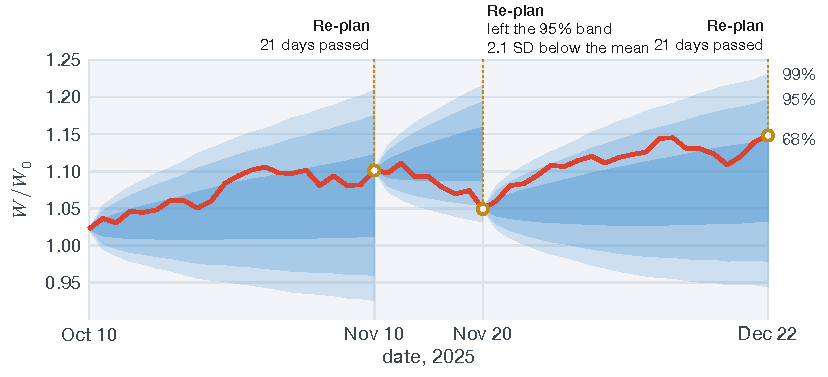
\includegraphics[width=0.9\textwidth]{figs/main/fig_mpc.pdf}
    \caption{\textbf{One episode of the rebalancing controller on real prices, 10 October to 22 December 2025.}
    The red line is the wealth $W$ of one backtest (the hand-picked $13$ names, Cobb--Douglas weighting, market
    hedge off, seed $5660$) divided by its initial wealth $W_0$. At each re-plan the controller projected $1{,}000$ paths of a
    multi-asset geometric Brownian motion $21$ trading days ahead; the nested cones are the $68$, $95$ and $99\%$
    bands of the projected portfolio value. The first and third re-plans came when $21$ trading days had passed.
    The second came on 20 November, when wealth left the $95\%$ band, $2.1$ standard deviations below the projected
    mean.}
    \label{fig:mpc}
\end{figure}

% talk/data/realrun_grid.csv, realrun_bars.csv, realrun_refs.csv
\begin{figure}[H]
    \centering
    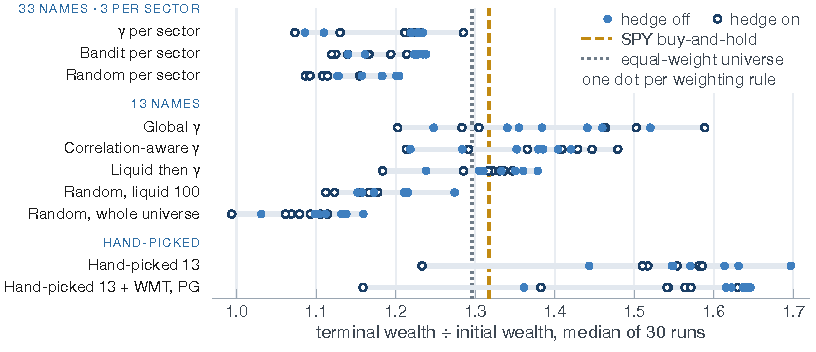
\includegraphics[width=\textwidth]{figs/main/fig_realrun.pdf}
    \caption{\textbf{Real-data backtest: terminal wealth by selection rule and weighting rule, 2 January 2025 to
    4 September 2026.} Each row is one selection rule, grouped by basket size ($33$ names, three per sector; $13$
    names; and the hand-picked lists of $13$ and $15$ names). Each dot is one of the seven weighting rules
    (Cobb--Douglas, CES on shares, CES on weights, Stone--Geary, minimum variance, tangency, and $130/30$
    long-short), placed at the median over $30$ runs (seeds $5660$--$5689$) of terminal wealth divided by initial
    wealth. Filled dots have the market hedge off and open dots have it on; with the hedge on, each re-plan capped portfolio beta
    at a level that was lower when the market was weaker, and up to five stocks with zero or negative beta could be held. The pale bar
    spans each row's lowest to highest dot. The dashed gold line is SPY buy-and-hold ($1.32$) and the dotted line is the equal-weight universe
    ($1.30$).}
    \label{fig:realrun}
\end{figure}

% talk/data/sf_density.csv, sf_qq.csv, sf_abs_acf.csv, sf_summary.csv
\begin{figure}[H]
    \centering
    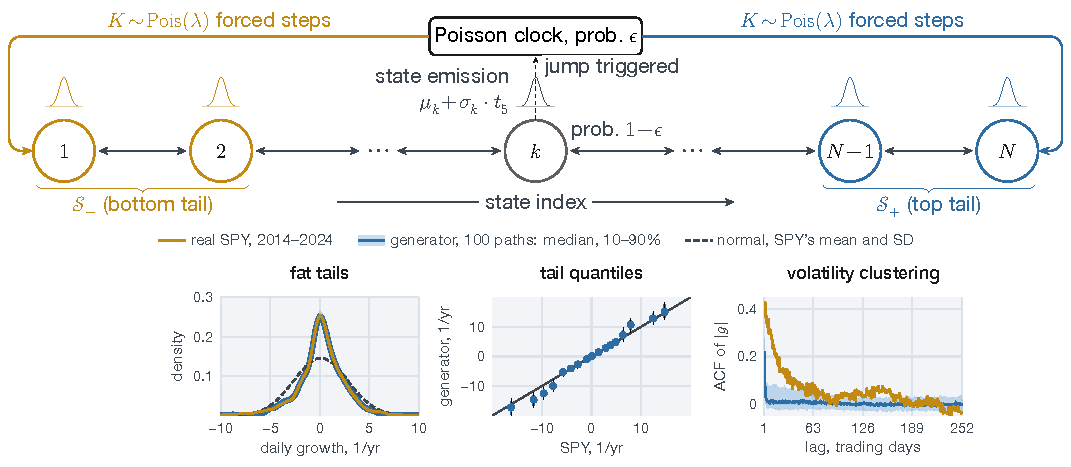
\includegraphics[width=\textwidth]{figs/main/fig_jumphmm.pdf}
    \caption{\textbf{The per-asset hidden Markov generator with jumps (JumpHMM) and its stylized facts for SPY.} Top: the generator's hidden
    states $1,\dots,N$ are ordered from the bottom to the top tail of the daily growth rate, and state $k$ emits
    $\mu_k + \sigma_k t_5$, a scaled Student-$t$ draw with five degrees of freedom. With probability $1-\epsilon$
    the chain moves by its fitted transition matrix; with probability $\epsilon$ a jump episode starts and lasts
    $K \sim \mathrm{Pois}(\lambda)$ forced steps, each drawn from the bottom tail set $\mathcal{S}_-$ or the top
    tail set $\mathcal{S}_+$~\citep{alswaidan2026variance}. Bottom: SPY's daily growth rates for 2014--2024 (gold)
    against $100$ generator paths (median line and $10$--$90\%$ band, blue) and a normal distribution with SPY's
    mean and standard deviation (dashed): the density, the generator's quantiles against SPY's, and the
    autocorrelation of the absolute growth rate $|g|$ out to $252$ trading days.}
    \label{fig:jumphmm}
\end{figure}

\begin{figure}[H]
    \centering
    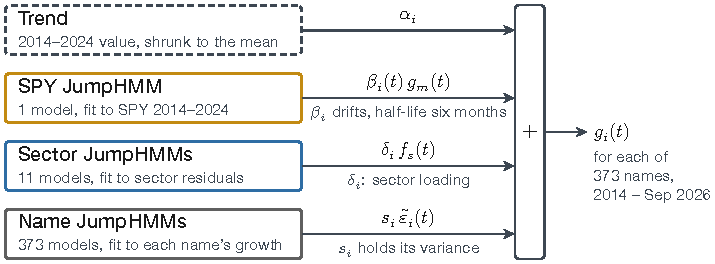
\includegraphics[width=0.85\textwidth]{figs/main/fig_multiasset.pdf}
    \caption{\textbf{Composition of one name's daily growth rate in the synthetic market.} Each name's growth rate
    $g_i(t)$ is the sum of a trend $\alpha_i$ (its 2014--2024 value, shrunk toward the cross-sectional mean), a
    market term $\beta_i(t)\,g_m(t)$ from one JumpHMM (hidden Markov generator with jumps) fit to SPY, a sector term $\delta_i f_s(t)$ from one of $11$
    sector JumpHMMs fit to sector residuals, and a name term $s_i\tilde\varepsilon_i(t)$ from the name's own
    JumpHMM, scaled so that the sum holds the name's variance. The loading $\beta_i(t)$ drifts with a half-life of
    $126$ trading days. The name terms are drawn independently across names, so dependence across names enters only
    through the market and sector terms.}
    \label{fig:multiasset}
\end{figure}

% talk/data/syn_axes.csv, syn_{typical,burst_stress,bear_stress}_{dots,bars,refs}.csv
\begin{figure}[H]
    \centering
    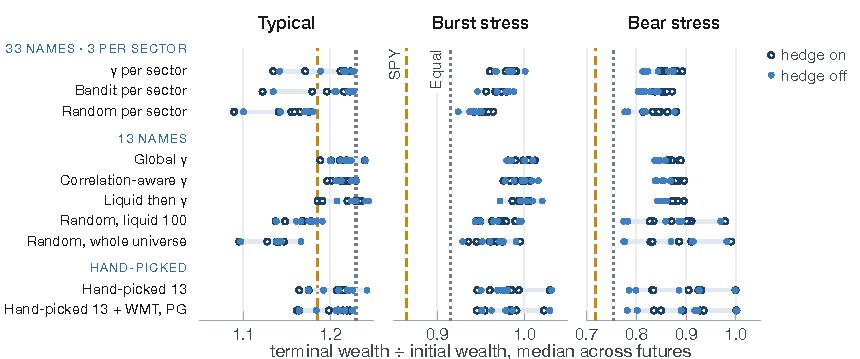
\includegraphics[width=\textwidth]{figs/main/fig_synthetic.pdf}
    \caption{\textbf{Terminal wealth on synthetic futures of the trading window, by selection rule and weighting
    rule.} The three panels are $600$ typical futures and two stress sets drawn from $10{,}000$ futures: the $200$
    with the deepest SPY drawdowns that contain a jump burst (burst stress), and the $200$ deepest without one (bear
    stress). Rows, dots, bars and lines are as in Fig.~\ref{fig:realrun}; each dot is the median across the set's
    futures (after a median over seeds within a future) of terminal wealth divided by initial wealth, and each panel has its own horizontal axis. SPY
    buy-and-hold ended at $1.19$, $0.86$ and $0.72$, and the equal-weight universe at $1.23$, $0.92$ and $0.75$, in
    the typical, burst-stress and bear-stress sets.}
    \label{fig:synthetic}
\end{figure}
